\begin{comment}
chapter 1: basics of lifetime patterns
chapter 2: aside for basics of memory management
chapter 3: time-space tradeoffs (optimization)
chapter 4: basics+optimizations -> requiremnts; how to implement these things
chapter 5: out of the box




feasibly recomputable state
for recomputable, either recompute every time, recompute some times, recompute
never

sharing pool; flyweight; shared immutable factory pattern (coding pattern)

inmemory designs; time-space tradeoffs; correlated lifetime

three risks: introduce leaks, create concurrency problems, extra space
consumption

\end{comment}

\chapter{Understanding Your Lifetime Requirements}
\index{Lifetime Requirements}

Your application needs some objects to live forever and it needs the rest to die
a timely death. Unfortunately, some of the important details governing memory
management are left in your hands. Java promised, with its automatic memory
management, that you could create objects without regard for the messy details of
storage allocation and reclamation. In Java, you needn't explicitly free objects,
which is at once the saviour from, and the source of, many problems with memory
consumption. Unless you are careful, your program will suffer from bugs such as
memory leaks\index{Memory Leaks}, race conditions, lock contention, or excessive
peak footprint. Furthermore, if your objects don't easily fit into the limits of
a single Java process, you will need to manage, explicitly, marshalling them in
and out of the Java heap.\index{Marshalling}

Very often, your application uses a data structure in a way that falls into one
of a handful of common \emph{lifetime requirements}\index{Lifetime Requirements}. The
nature of each requirement dictates how much help you will get from the Java runtime
in the desired preservation and reclamaion of objects, and where it leaves you to
your own devices. 

An important step in the design process of any large application is understanding
the lifetime requirement for each of your data models. In this chapter, we
describe the five common lifetime requirements: objects needed only transiently,
objects needed for the duration of the run, objects whose lifetime ends along
with a method invocation, objects whose lifetime is tied to some other object,
and, most difficult of all, objects that live or die based on need.
\autoref{tab:five-lifetimes} summarizes these five important requirements. We step
you through each of the requirements, defining them and giving examples of how to
know when you have an instance of each.

\begin{table}
\centering
%	\begin{tabular}{lp{0.30\textwidth}p{0.35\textwidth}}
	\begin{tabular}{ll}
	\toprule
	  %&
	   Lifetime Requirement & Example \\ \cmidrule(r){1-1} \cmidrule(l){2-2}
	   %\cmidrule(r){2-2} \cmidrule(l){3-3}
	%\autoref{temporary-lifetime} &
	  Temporary & new parser for every date
	\\
	%\autoref{correlated-lifetime} &
	Correlated with Another Object & object annotations
	\\
	%\autoref{correlated-lifetime} &
	Correlated with a Phase or Request & tables needed only for parsing
	\\
	%\autoref{deferred-deletion} &
	Request/phase-spanning & session state 
	\\
	%\autoref{forever-lifetime} &
	 Permanently Resident & product catalog
	\\
%	\autoref{correlated-lifetime-2} & {Correlated with Phase} &
%	DOM used only for parsing
%	\\
	%\autoref{deferred-deletion} &
	 Time-space Tradeoff & database connection pool
	  \\
%period\\ scoped to a phase/request\\
%correlated with an object (annotations)\\
%correlated with need}\\ \hline
%reusable & maybe i'll need it later \\ \hline
	\bottomrule
	\end{tabular}
	\caption{Common requirements for the lifetime of objects that your
	application must implement properly, in order to avoid correctness or
	performance problems.}
	\label{tab:five-lifetimes}
\end{table}

\begin{figure}
\centering
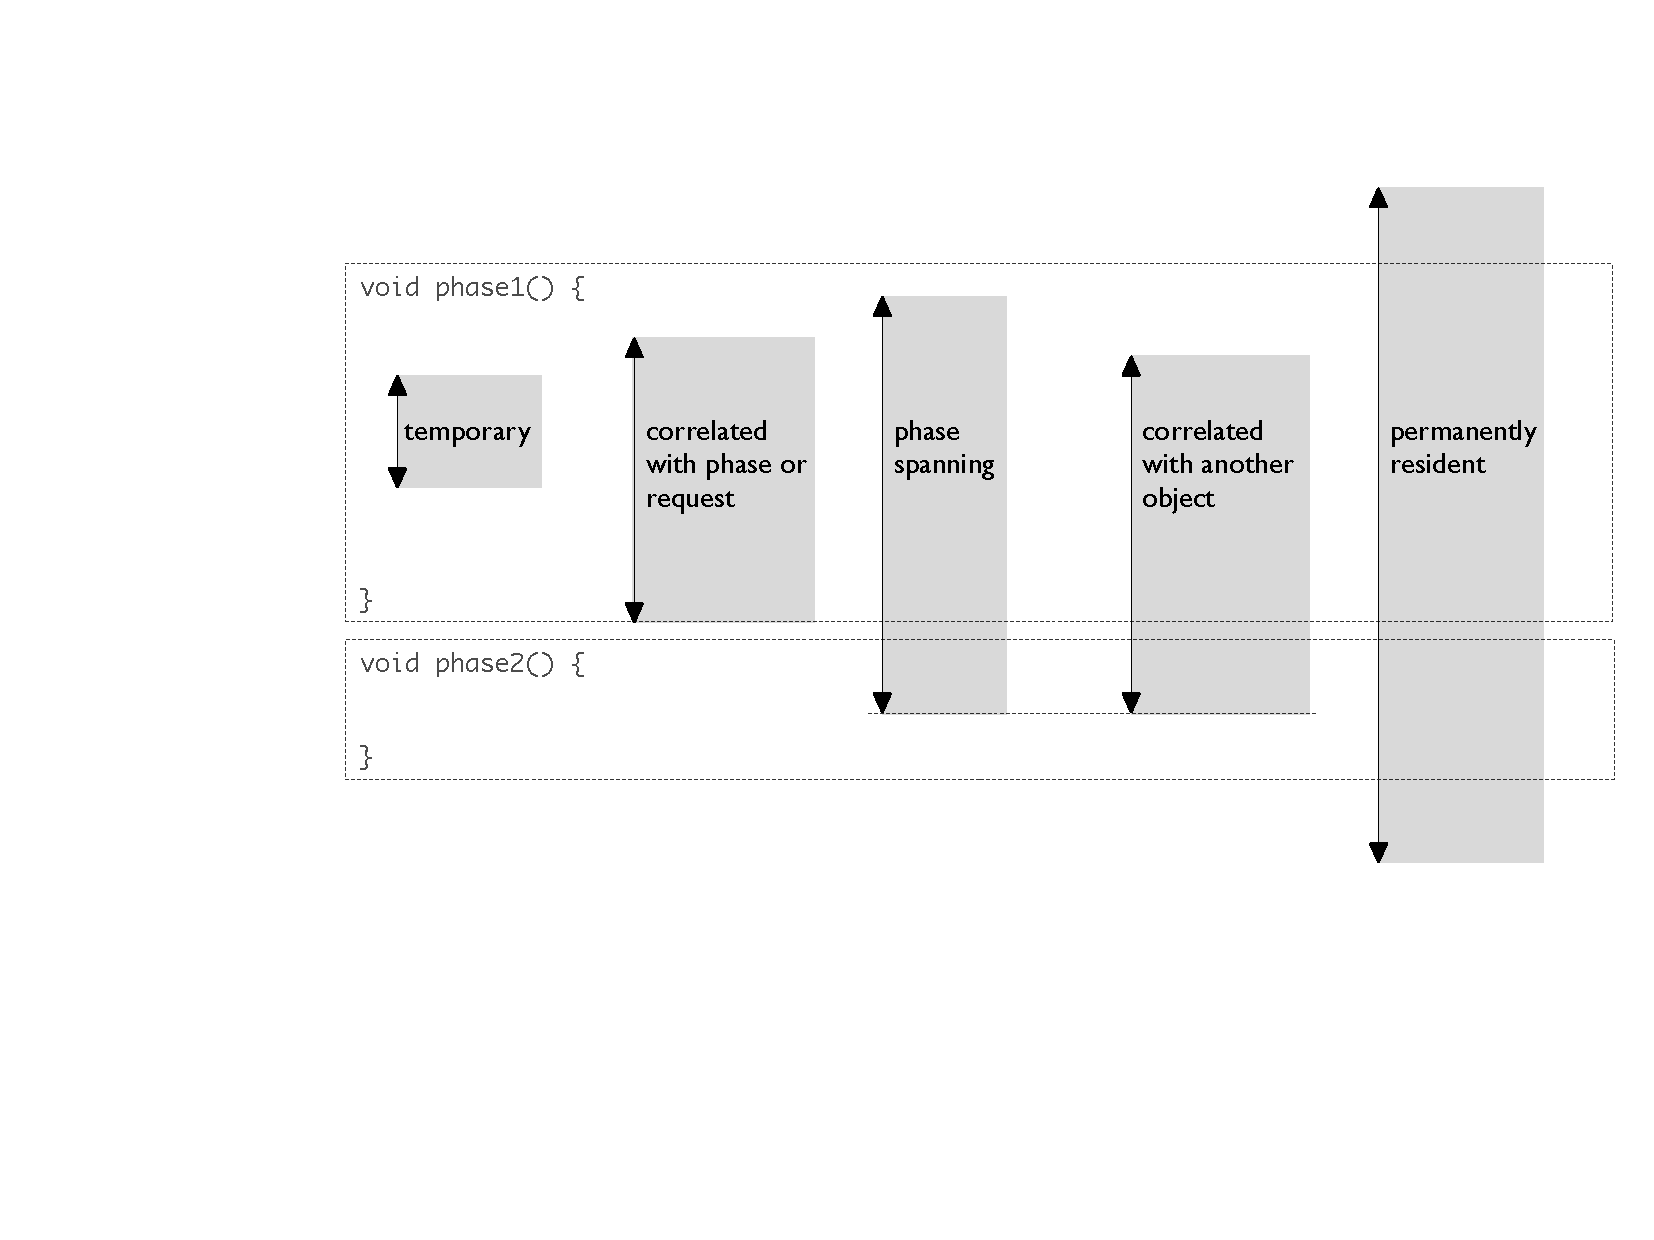
\includegraphics[width=\textwidth]{part4/Figures/requirements}
\caption{Illustration of some common lifetime requirements.}
\label{fig:five-lifetimes}
\end{figure}

Once you have mapped out the lifetime requirements of your data models, the next
step is to chose the right implementation details in order to correctly implement
each requirement. The remaining chapters in this part show how to implement these
requirements.

%The trickier aspects of memory management, summarized in
%\autoref{tab:tricky-memory-management}, are discussed in greater detail in
%later chapters.


\section{Object Lifetimes in A Web Application Server}

%Configuring memory settings is an iterative process. It usually involves a
%fair amount of trial and error, as one tunes the various knobs to balance memory
%consumption and application performance. These knobs affect things like the size of the Java
%heap, how many entries a cache should hold, and the timeout value for these
%caches. This is usually a process of black box tuning: twist a knob, and see
%how overall performance changes. In addition to being hit
%and miss, it is also quite prone to bugs. If you set the size of a cache too
%high, you risk poor performance due to excessive garbage collection, and even
%possibly process failures, due to running out of heap space.

To introduce the common requirements for object lifetime, we walk through several
scenarios found in most long-running server applications. These applications
provide an interesting case study for lifetime management. Managing lifetime when
the application runs forever is an especially complex issue. This is true for
more than for servers alone. Desktop applications such as the Eclipse integrated
development environment shares many of the same challenges. Improperly managing
the lifetimes of objects, for short-running applications, often does not result
in critical failure. Indeed, the application often finishes its run before one
would even notice a problem with memory consumption. Plus, you're probably don't
run many instances of a short-running application simultaneously; and so
achieving the ultimate in scalability is not a primary concern. In contrast, if
an application runs more or less forever, then mistakes pile up over time. In
addition, caching plays a large role in these applications, since they often
depend on data fetched from remote servers, or from disk, neither of which can
support the necessary throughput and response time requirements. The ability for
mistakes to pile up, and for misconfigured or poorly implemented caches to impede
performance means that special care must be taken when implementing your server application.

The heap consumption of this application will fluctuate over time. A timeline
view of expected memory consumption helps to visualize these changes. It
visualizes memory during the lulls and peaks of activity, as requests are
processed and when sessions time out, and as the server starts up. We will use
these over the next few pages, as we walk through the common cases of lifetime
requirements.




% \begin{example}{Lifetime in A Web Application Server}
To help introduce the common lifetime requirements, we walk through an example of
a shopping cart server application. The server, on startup, preloads catalog data
into memory to allow for quick access to this commonly used data. It also
maintains data for users as they interact with the system, browsing and buying
products. Finally, it caches the response data that comes from a remote service
provider that charges per request. The remainder of this chapter walks you
through understanding the lifetime requirements of these data structures.
% How does Java heap consumption vary over time? Which heap size fluctuations
% indicate a problem, and which are expected behavior? \end{example}

\begin{figure}
	\centering
	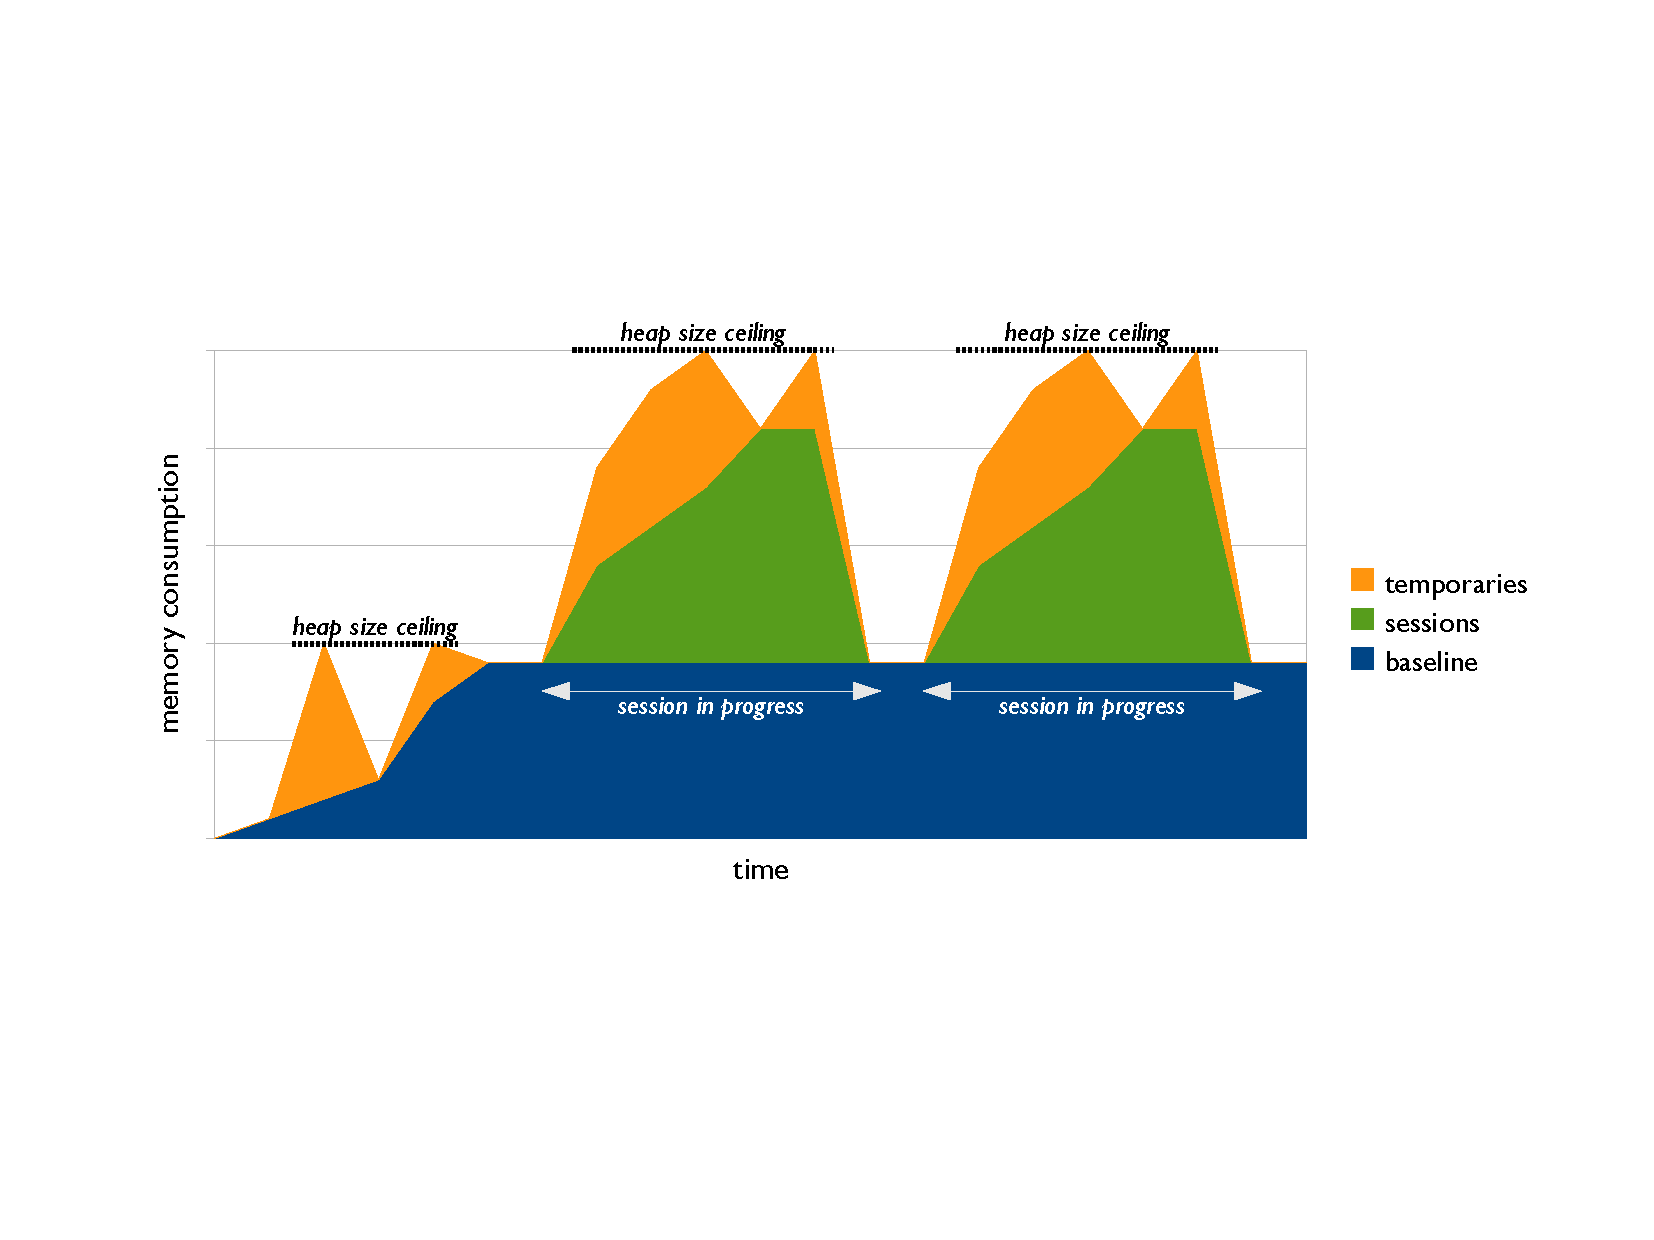
\includegraphics[width=\textwidth]{part4/Figures/lifetime/timeline-base-session-temps}
	\caption{Memory consumption, over time, typical of a web application server.}
	\label{fig:timeline-base-session-temps}
\end{figure}

\section{Lifetime Requirement: Permanently Resident}
\label{sec:forever-lifetime}
\index{Permanently Resident Objects}

\autoref{fig:timeline-base-session-temps} shows the timeline of memory
consumption of our example server 
during and shortly after its initial startup.
During the startup interval, the server preloads catalog data into
the Java heap. Then, the server is warmed with with two test requests.
The total height of the area
under the curves represents the memory consumption at that point in time. 
The preloaded catalog
data will be used for the entire duration of the server process.
\index{Objects That Live Forever}
Therefore, the Java objects that represent this catalog are objects that are
needed forever. In the timeline picture, this data is respresented by the lowest area, labeled
\emph{baseline}. Notice how it ramps up quickly, and then, after the server has
reached a ``warmed up'' state, memory consumption of this baseline data evens out
on a plateau for the remainder of the run.

\subsection{Permanently Resident Objects in Practice}

In the above example, a \class{DateFormat} object was created in every loop
iteration and used only once. We can improve this situation by creating and using
a single formatter for the duration of the run. The Java API documentation, in
writing at least, encourages this behavior, but leaves the burden of doing so on
you. You must be careful to remember that it is not safe to do so in multiple
threads. The next chapter will discuss remedies to this problem. The updated code
for the \code{parse} method would be:

\begin{shortlisting}
static final DateFormat fmt = new DateFormat.getInstance();

Date parse(String string) {
	return fmt.parse(string, new ParsePosition(0));
}
\end{shortlisting} 


\section{Lifetime Requirement: Request-spanning}
\index{Session State}
After the server is warmed up, it begins to process client requests. Imagine
interacting with a commerce site with a web browser. First you browse around,
looking for items that you like, and add them to your shopping cart. Eventually,
you may authenticate and complete a purchase. As you browse and buy, the server
maintains some state, to remember aspects of what you have done so far. For
example, the server stores the incremental state of multi-step transactions,
those that span multiple page views.
 This session
state, at least the part of it stored in the Java heap, will go away soon after
your browsing session is complete. In the timeline figure, this portion of memory
is labeled \emph{sessions}. It ramps up while a session is in progress, and then,
in the example illustrated here, soon all of that session memory should be
reclaimed.

\section{Lifetime Requirement: Temporaries}
\label{sec:temporary-lifetime}
\index{Temporary Objects}

The catalog data and session state are both examples of objects that are expected
to stick around for a while. In the course of preloading the cache and responding
to client requests, the server application will create a number of objects that
are only used for a very short period of time.
They help to faciliate the main
operations of the server. These temporary objects will be reclaimed by the \jres
garbage collector in relatively short order. The point at which an object is
reclaimed depends on when the garbage collector notices that it is reclaimable.
Normally, the garbage collector will wait until the heap is full, and then
inspect the heap for the objects that are still possibly in use. In this way, the
area under the \emph{temporaries} curve has a see-saw shape. As the temporaries
pile up, waiting for the next garbage collection, they contribute more and more
to memory footprint. Normally, once the \jre runs a garbage collection, these
temporaries no longer in use will no longer contribute to heap consumption.

In this way, temporary objects
\emph{fill up the headroom} in the heap.\index{Heap Headroom} If there is a
large amount of heap space unused by the longer-lived objects, then the
temporaries can be reclaimed less often. This is a good thing, because a
garbage collection is an expensive proposition.
\index{Heap Size Settings} \index{Maximum Heap Size} \index{-Xmx}
When configuring your application, you may specify a maximum heap size. It
should certainly be larger than the baseline and session data. How much
larger than that? This choice directly affects the amount of \emph{headroom},
 that is the amount of space available for temporaries to pile up.

\subsection{Temporaries in Practice}
If your application is like most Java applications, it creates a large number of
these temporary objects. They hold data that will only be used for a very short
interval of time. It is often the case that the objects in these transient data
structures are only ever reachable by local variables. For example, this is the
case when you populate a \class{StringBuilder}, turn it into a \class{String},
and then ultimately (and only) print the string to a log file. The point at
which these objects, the string builder, string, and character arrays, are no
longer used is only shortly after they are constructed:

\begin{shortlisting}
String makeLogString(String message, Throwable exception) {
	StringBuilder sb = new StringBuilder();
	sb.append(message);
	sb.append(exception.getLocalizedMessage());
	return sb.toString();
}
void log(String message, Throwable exception) {
	System.err.println(makeLogString(message, exception));
}
\end{shortlisting}

A temporary object serves as a transient home for your data, as it makes its way
through the frameworks and libraries you depend on. Temporaries are often
necessary to bridge separately developed code and enable code reuse. The above
example avoids code dupliation and ensures uniformity of the output data by
factoring out the logic of formatting messages into the \code{makeLogString}
method.

%By converting your data layout into a form that an API requires,
%then you can reuse the functionality it provides.

In many cases, the \jre will do a sufficient job in managing these temporary
objects for you. Generational garbage collectors \index{Generational Garbage
Collection} these days do a very good job digesting a large volume of temporary
objects. In a generational garbage collector, the \jre places temporary objects
in a separate heap, and thus need only process the newly created objects, rather
than all objects, during its routine scan.

There are two potential problems that you may encounter with temporary objects.
The first is the runtime cost of initializing the state of the temporary
objects' fields. Even if allocating an freeing up the memory for an object is
free, there remains the work done in the constructor:

\begin{shortlisting}
class Temp {
	private final Date date;
	
	public Temp(String input) { /* constructor */
		this.date = DateFormat.getInstance().parse(input);
	}
}
\end{shortlisting}

Even if an instance of \class{Temp} lives for only a very short time, its
construction has a high cost. It is often the case that this expense is hidden
behind a wall of APIs. If so, then what you think of as trivial temporary (since
you, after all, are in control of when the instance of \class{Temp} lives and
dies), would in actuality be far from trivial in runtime expense. Expenses can
pile up even further if temporary object constructions are nested.

There is a second potential problem with temporary objects. By creating temporary
objects at a very high rate, it is possible to overwhelm either the garbage
collector, or the physical limitations of your hardware. For example, at some
point, the memory bandwidth necessary to initialize the temporary objects will
exceed that provided by the hardware. Say your application fills up the temporary
heap ever second. In this case, based on the common speeds of garbage collectors,
your application could easily
 spend over 20\% of its time collecting garbage. Is it difficult to fill up the
 temporary heap once per second? Typical temporary heap sizes run around 128
 megabytes. Say your application is a serves a peak of 1000 requests per second,
 and creates objects of around 50 bytes each. If it creates around 2500
 temporaries per request, then this application will spend 20\% of its time
 collecting garbage.


%A great many of these
%temporary structures serve the role of a kind of lubricant, making it easy for
%you to write code that ties together the separately written parts of your code
%base and reuses standard libraries as much as possible. Often, these are
%objects that are not a fundamental necessity of what you're trying to
%accomplish. If
%you had the freedom to code highly specialized implementations of the important
%cases, from scratch, many of these temporary structures would be unnecessary.

\begin{example}{How Easy it is to Create Lots of Temporary Objects}
A common example of temporaries is parsing
and manipulating data coming from the outside world. Identify the temporary
objects in the following code.
% to the wire?

\begin{shortlisting}%[float,caption=Code that constructs 8 temporary objects tohandle two dates.,label=TempExampleCode]
void main(String xy) {
	doWork(xy.substring(0,10), xy.substring(10));
}	
void doWork(String x, String y) {
	doRemoteProcedureCall(parse(x));
	doRemoteProcedureCall(parse(y));
}
Date parse(String string) {
	return DataFormat.getInstance().parse(string, new ParsePosition(0));
}
void doRemoteProcedureCall(Date date) {
	long timestamp = date.getTime();
	...
}
\end{shortlisting}
\end{example} 

This code starts in the \code{main} method by splitting the input string into two
substrings. So far, the code has created four objects (one \class{String} and one
character array per substring). Creating these substrings makes it easy to use
the \code{doWork} method, which takes two Strings as input. However, observe that
these four objects are not a necessary part of the computation. Indeed, these
substrings are eventually used only as input to the \class{DateFormat}
\code{parse} method, which has been nicely designed to allow you to avoid this
very problem. By passing a \class{ParsePosition}, one can parse substrings of a
string without having to create temporary strings (at the expense of creating
temporary \class{ParsePosition} objects).


\begin{figure}
	\centering
	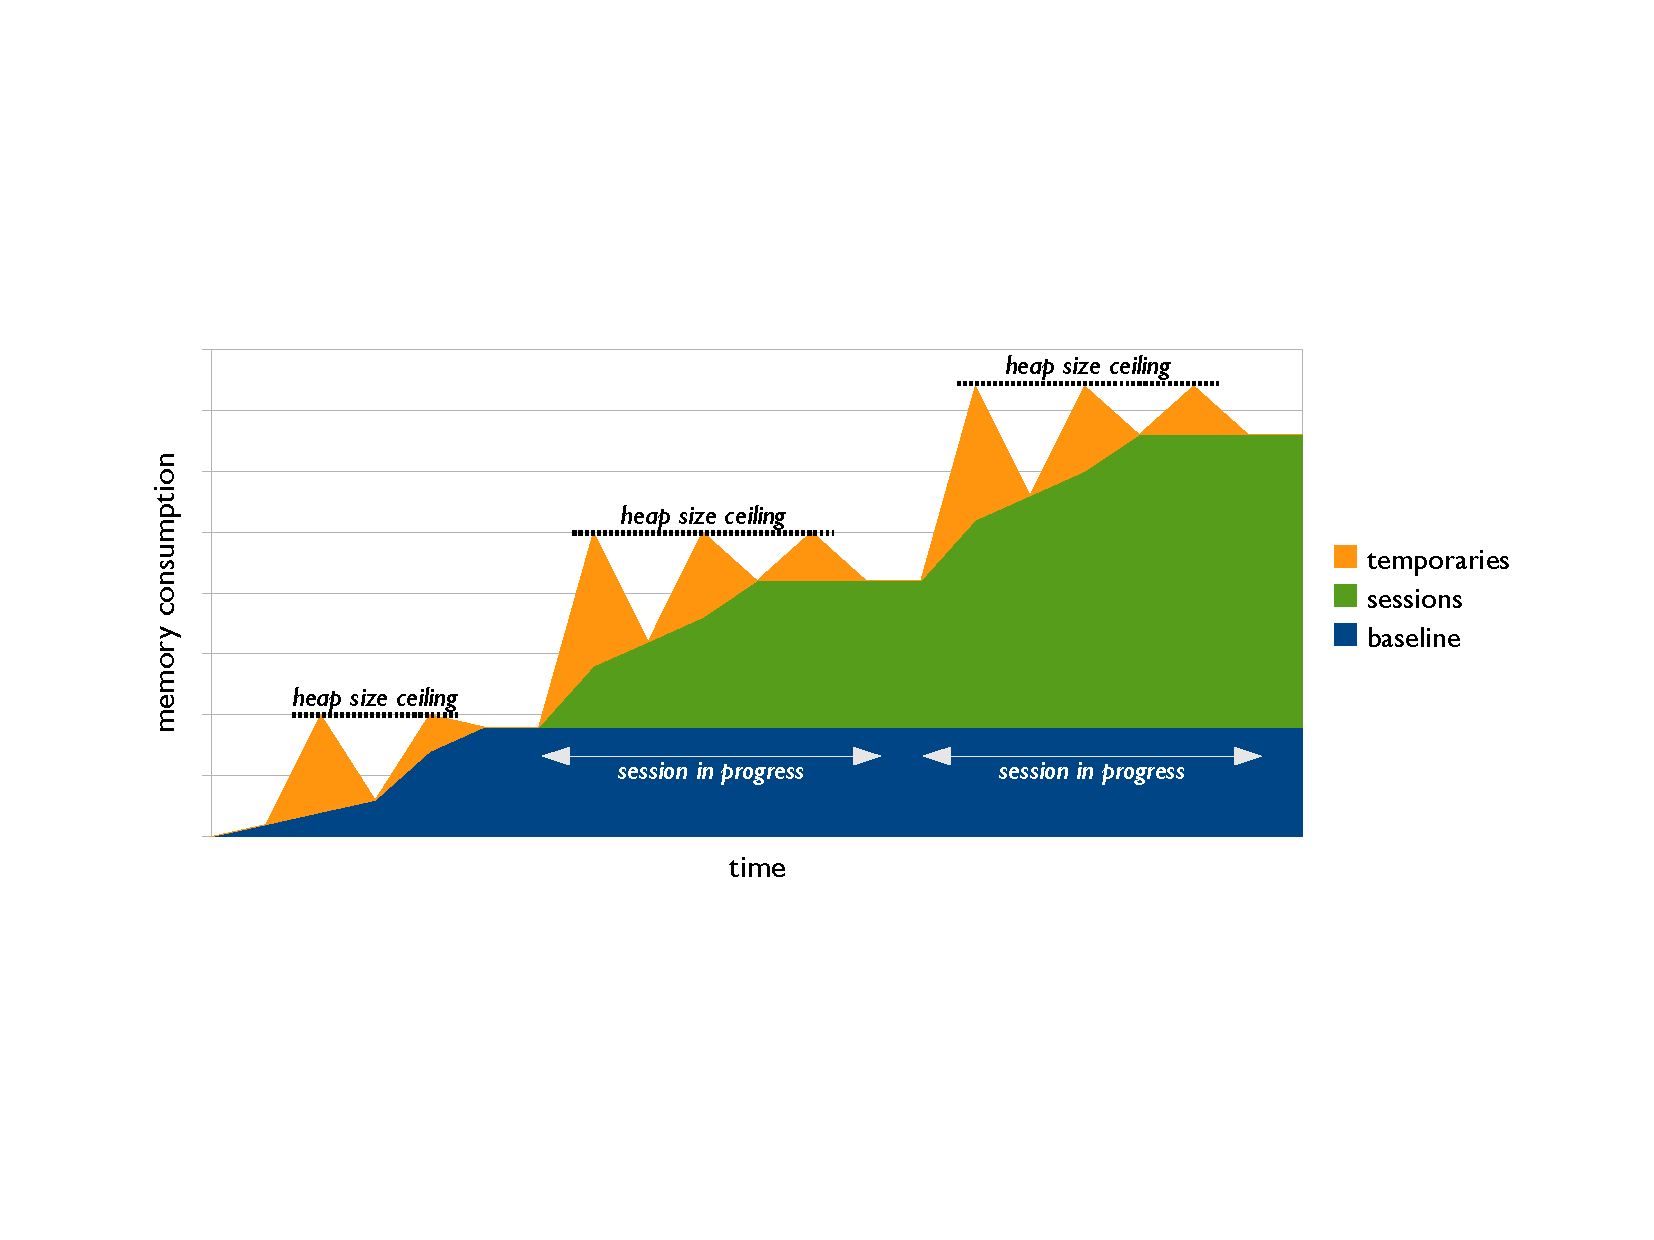
\includegraphics[width=\textwidth]{part4/Figures/lifetime/timeline-base-session-temps-with-leak}
	\caption{If session state is not cleaned up
	properly, a memory leak is the result. This means more frequent garbage
	collections, and ever increasing heap size.}
	\label{fig:timeline-base-session-temps-with-leak}
\end{figure}

\section{Lifetime Requirement: Correlated Lifetime}
\label{sec:correlated-lifetime}
\index{Memory Leaks}

The catalog data should last forever, while the
session data lives for some bounded period of time. It is possible that session
state will live beyond the end of your session, but nonetheless it has a
lifetime that is bounded. If, due to an bug, part of this session state is not
reclaimed, the application will leak memory. Though it is supposed to have a bounded lifetime, it
\marginpar{\textbf{Memory Leaks} are still possible, even with
automatic garbage collection!} 
accidentally lives forever. In this
case, over time, the amount of heap required for the application to run will increase without bound.
\autoref{fig:timeline-base-session-temps-with-leak} illustrates this situation,
in the extreme case when all of session state leaks. Over time, the area under
the curve steps higher and higher.

%As you scan the timeline from left to right, memory consumption 
%it fetches catalog data from its database, and stores them in the Java heap. 

\subsection{Correlated Lifetime in Practice}

Many objects are needed for a bounded interval of time. In some cases, this
interval is bounded by the lifetime of another object. In a second important
scenario, the lifetime of an object is bounded by the duration of a method call.
Once that other object is not needed, or once that method returns, then these
\emph{correlated} objects are also no longer needed. These are the two important
cases of objects with correlated lifetime.

\paragraph{Objects that Live and Die Together}
\label{sec:correlated-lifetime-1}

Normally, if you need to augment the state stored an object, you modify
the source code of some existing classes. For example, to add a secondary
mailing address to a \class{Person} object, you can add a field to that class, and update the
initialization and marshalling logic accordingly. Sometimes, you will find it
necessary to associate information with an object that is, for one reason or the
other, locked down.

\begin{example}{Annotations}
In order to debug a performance problem, you need to associate a timestamp with
another object. Unfortunately, you don't have access to the source code for
that object's class. Where do you keep the new information, and how can you
link the associated storage to the main objects without introducing memory
leaks?\index{Memory Leaks}
\end{example}

If you can't modify the class definition for that object, then you will have to
store the extra information elsewhere. These \emph{side annotations}\index{Side
Annotations} will be objects themselves, and you need to make sure that their
lifetimes are correlated with the main objects. When one dies, the other
should, too.

You could store the annotations in a map that is keyed by the
original object, say of type \class{T}:

\begin{shortlisting}
Map<T, Date> timestamps = new HashMap<T, Date>();

void addTimestamp(T t) {
	timestamps.put(t, new Date());
}
Date getTimestamp(T t) {
	return timestamps.get(t);
}
\end{shortlisting}

This solution will function correctly, but suffers from a \emph{memory
leak}\index{Memory Leak}. As the application runs, it will consume greater
amounts of Java heap, up until the point when the \jre runs out of heap space to
allocate any more objects. This solution leaks memory, because the
\code{timestamps} map introduces a reference to the main objects. When the
garbage collector scans the heap to see which objects are still alive, the
references in this map will be among those that keep the objects alive. The next
chapter discusses these issues in more detail. An improved solution would use the
\class{WeakHashMap} from the Java standard libraries. By replacing the
initialization of the \code{timestamps} map, we have the same functionality as
before, but no memory leak.

\begin{shortlisting}
Map<T, Date> timestamps = new WeakHashMap<T, Date>();
\end{shortlisting}

Note that this same situation can hold even if you are able to modify the class
definition. A common scenario requires annotations on only a subset of all
instances of a class. In this case, is it not worth paying the memory cost to
have the ability to annotate every single instance. Therefore, this is another
case where a solution of side annotations, stored in a \class{WeakHashMap},
shines.

\paragraph{Objects that Live and Die with Program Phases}
\label{sec:correlated-lifetime-2}

Similar to the way the lifetime of an object can be correlated with another
object, lifetimes are often correlated with method invocations. When a method
returns, objects correlated with it should go away. For temporary objects, this
is usually easy to ensure, since they are usually only reachable from stack
locations. For the medium-to-long running methods that implement the
core functionalities of the program, this correlation is harder to get right.

For example, if your application loads a log file from disk,
parses it, and then displays the results to the user, it has roughly three
phases for this activity. Most of the objects allocated in one phase are scoped to that
phase; they are needed to implement the logic of that phase, but not subsequent
phases. The phase that loads the log file is likely to maintain maps that
help to cross reference different parts of the log file. These are necessary
to facilitate parsing, but, once the log file has been loaded, these maps can be
discarded. In this way, these maps live and die with the first phase of this
example program. If they don't, because the machinery you have set up to
govern their lifetimes has bugs, then your application has a memory
leak\index{Memory Leaks}.

This lifetime scenario is also common if your application is an
server that handles web requests.

\begin{example}{Memory Leaks in an Application Server}
	A web application server handles servlet requests. How is it possible that
	objects allocated in one request would unintentionally survive beyond the end
	of the request?
\end{example} 
  
In server applications, most
objects created within the scope of a request should not survive the
request. Most of these \emph{request-scoped}
\index{Request-scoped Lifetime} objects are not used by the application after the
request has completed. In the absence of application or framework bugs, they will
be collected as soon as is convenient for the runtime. In this example, the
lifetime of objects during a request are \emph{correlated} with a method
invocation: when the servlet \class{doGet} or \class{doPut} (etc.) invocations
return, those correlated objects had better be garbage collectible.

\index{Memory Leaks: Why?}
There are many program bugs and configuration missteps that can lead to
problems. The general problem is that a reference to an object stays around
indefinitely, but becomes
\emph{forgotten}, and hence rendered unfindable by the normal application
logic. If this request-scoped data structure were only reachable from stack
locations, you would be fine. Therefore, a request-scoped object will leak only
when there exist references from some data structure that lives forever. Here
are some common ways that this happens.

\begin{itemize}
  \item Registrars, where objects are registered as listeners to some service,
  but not deregistered at the end of a request.
  \item Doubly-indexed registrars. Here the outer map provides a key to index
  into the inner map. A leak occurs when the outer key is mistakenly
  overwritten mid-request. This can happen if the namespace of keys isn't
  canonical and two development groups use keys that collide. It can also
  happen if there is a mistaken notion, between two development groups, of who
  owns respnsibility of populating this registrar.
  \item Misimplemented hashcode or equals, which foils the retrieval of an
  object from a hash-based collection. If developers checked the return value of
  the \code{remove} method, which for the standard collections would indicate a failure to remove, then
  this bug could be easily detected early; but developers tend not to do this.
\end{itemize}

The next chapter goes into greater detail on how to avoid these kinds of
errors. \autoref{chapter:tools} describes tooling that can help you
detect and fix the bugs that make it into your finished application.

\section{Lifetime Requirement: Time-space Tradeoffs}
\index{Time-Space Tradeoffs}
Finally, this example server caches data from some expensive third-party data
source. When caching data inside of Java objects, there is a fourth effect on
the timeline landscape. The
cached data must be configured properly to live long enough to be useful. It
also must not occupy so much of the heap so as to leave little headroom for
temporaries. \autoref{fig:timeline-base-session-temps-with-cache} shows an
example where the cache has probably been configured to occupy too much heap
space. Observe how, compared to the other timeline figures, there is little
headroom for temporaries. In this case, the result is more frequent garbage
collections. If the cache were sized to occupy an even greater amount of heap
space, it is possible that there would no longer be room to fit session data.
The result in this case would be failures in client requests. 
Sizing caches is important, but tricky to get right.

\begin{figure}
	\centering
	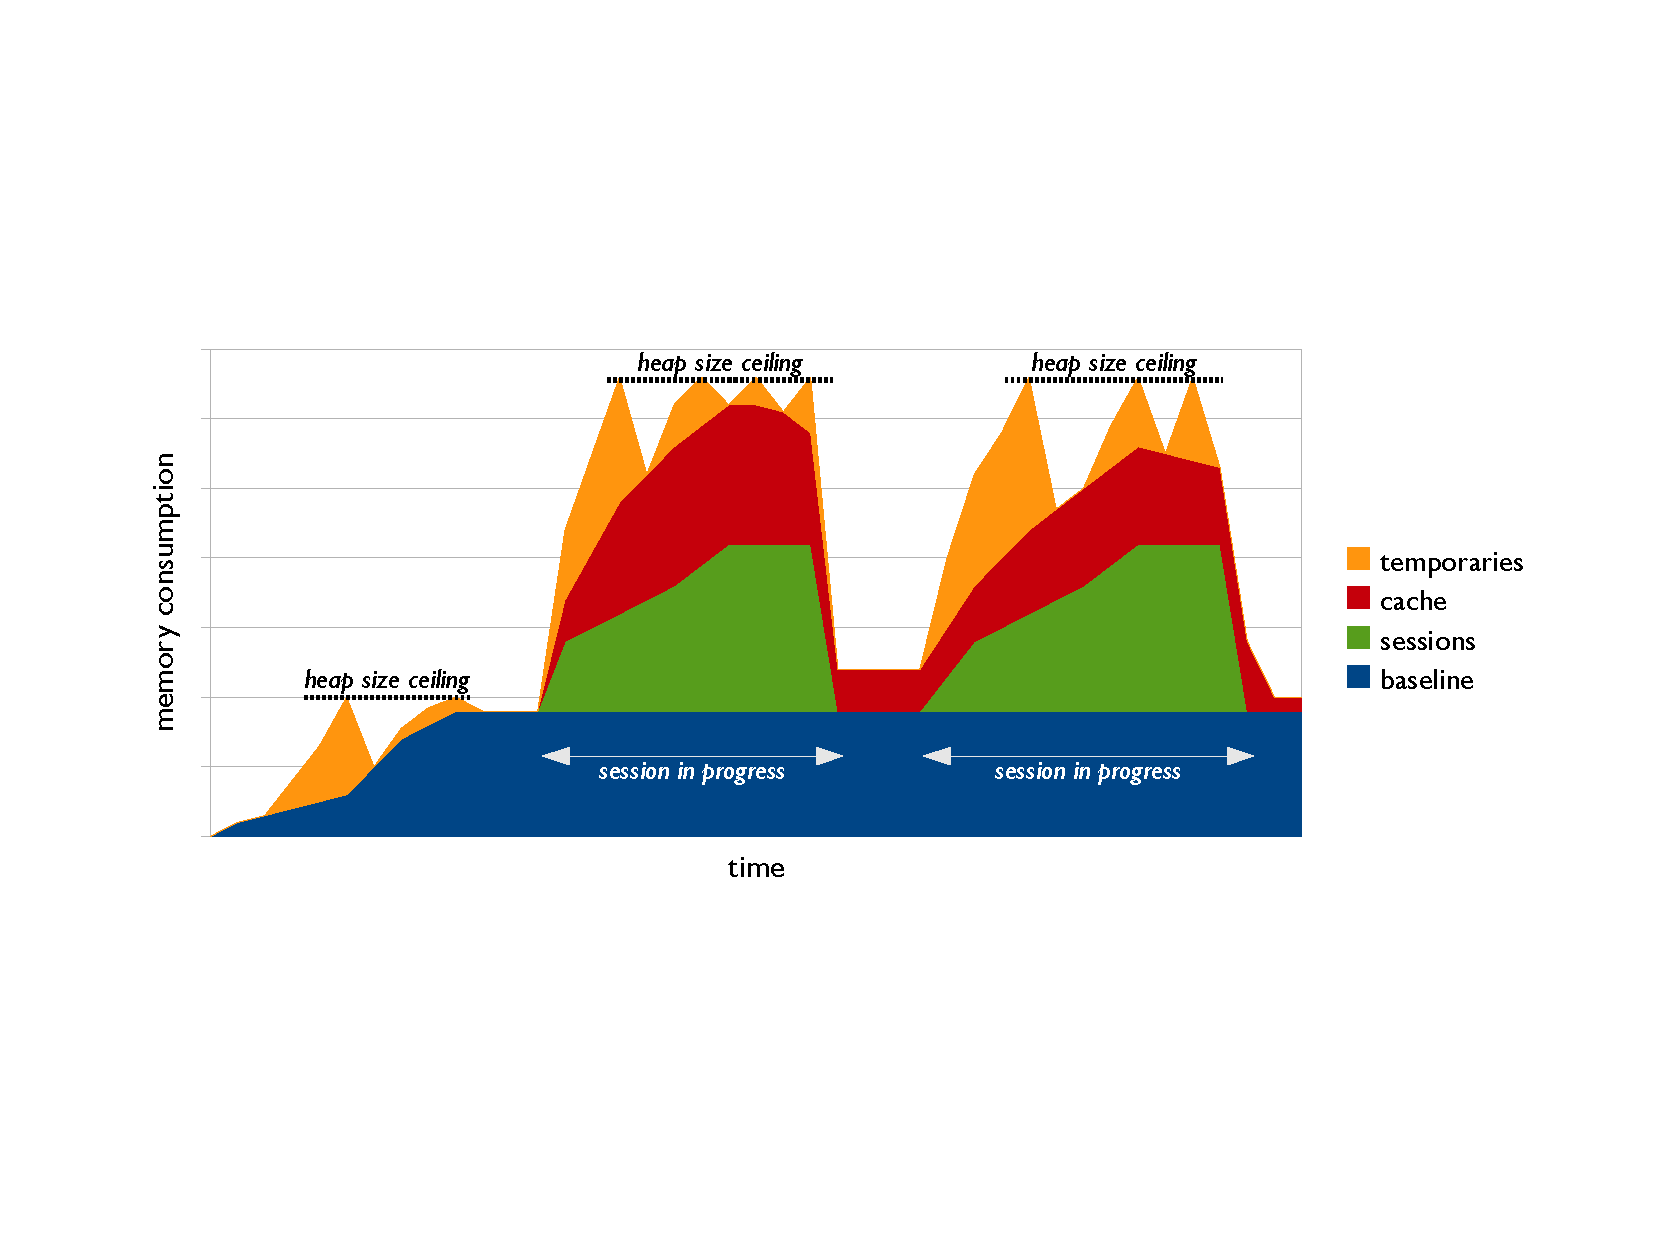
\includegraphics[width=\textwidth]{part4/Figures/lifetime/timeline-base-session-temps-with-cache}
	\caption{When a cache is in use, this leaves less headroom for temporary
	object allocation, often resulting in more frequent garbage collections.}
	\label{fig:timeline-base-session-temps-with-cache}
\end{figure}

% introduced by example in this chapter, and
%Many objects are either temporaries or needed for
%the entire run of your application. Sometimes you create objects whose lifetime
%is correlated with other objects or that should go away when a method
%invocation completes. Sometimes you need to manage objects hanging around
%longer than their current need, to avoid future recomputations or refetching
%of data in the case when it is needed in the near future. 

%\begin{table}
%\centering
	%\begin{tabular}{ll} \toprule
    %%%%	%& Things Java Doesn't Do Automatically \\ \cmidrule{2-2}
%    	\autoref{avoiding-lifetime-bugs} & {Avoiding Memory Leaks} \\
%    	\autoref{balance-time-and-space} & {Balancing Time and Space} \\
%    	\autoref{outisde-java-box} & {Supporting Massive Data Sets}  	\\
%        \bottomrule
%    \end{tabular}
%	\caption{The tricky aspects of memory management.}
%	\label{tab:tricky-memory-management}
%\end{table}




% correlated with need: as soon as last user goes away, remove his stuff 
% share common expressions to save space, but using strong references -> memory
% leak; plugins in eclipse go away when all views
% sharing pool 

% weak ref keys -> annotation
% weak ref values -> sharing pool

% soft ref values -> caching

% annotation by map lookup




\section{Objects that Span Program Phases or Requests}
\label{sec:correlated-with-need}

Some objects need to be kept around for operations that span several independent
operations, or are used across multiple threads. They are used beyond the scope
of a phase, are not correlated with another object, but don't live forever. 





%% OLD STUFF NMM 20090820
%\section{Request Scoping}
%\section{Correlated Lifetime}
%\paragraph{Weak and Soft references in Java}
%\section{Memory Leaks and Drag}
%\section{Examples}
%\subsection{Transient Near-Copies}
%\subsubsection{String Canonicalization}
%\subsection{Temporary Collections}
%\subsection{Facilitators}
